\documentclass[floatsintext,man]{apa6}

\usepackage{amssymb,amsmath}
\usepackage{ifxetex,ifluatex}
\usepackage{fixltx2e} % provides \textsubscript
\ifnum 0\ifxetex 1\fi\ifluatex 1\fi=0 % if pdftex
  \usepackage[T1]{fontenc}
  \usepackage[utf8]{inputenc}
\else % if luatex or xelatex
  \ifxetex
    \usepackage{mathspec}
    \usepackage{xltxtra,xunicode}
  \else
    \usepackage{fontspec}
  \fi
  \defaultfontfeatures{Mapping=tex-text,Scale=MatchLowercase}
  \newcommand{\euro}{€}
\fi
% use upquote if available, for straight quotes in verbatim environments
\IfFileExists{upquote.sty}{\usepackage{upquote}}{}
% use microtype if available
\IfFileExists{microtype.sty}{\usepackage{microtype}}{}

% Table formatting
\usepackage{longtable, booktabs}
\usepackage{lscape}
% \usepackage[counterclockwise]{rotating}   % Landscape page setup for large tables
\usepackage{multirow}		% Table styling
\usepackage{tabularx}		% Control Column width
\usepackage[flushleft]{threeparttable}	% Allows for three part tables with a specified notes section
\usepackage{threeparttablex}            % Lets threeparttable work with longtable

% Create new environments so endfloat can handle them
% \newenvironment{ltable}
%   {\begin{landscape}\begin{center}\begin{threeparttable}}
%   {\end{threeparttable}\end{center}\end{landscape}}

\newenvironment{lltable}
  {\begin{landscape}\begin{center}\begin{ThreePartTable}}
  {\end{ThreePartTable}\end{center}\end{landscape}}




% The following enables adjusting longtable caption width to table width
% Solution found at http://golatex.de/longtable-mit-caption-so-breit-wie-die-tabelle-t15767.html
\makeatletter
\newcommand\LastLTentrywidth{1em}
\newlength\longtablewidth
\setlength{\longtablewidth}{1in}
\newcommand\getlongtablewidth{%
 \begingroup
  \ifcsname LT@\roman{LT@tables}\endcsname
  \global\longtablewidth=0pt
  \renewcommand\LT@entry[2]{\global\advance\longtablewidth by ##2\relax\gdef\LastLTentrywidth{##2}}%
  \@nameuse{LT@\roman{LT@tables}}%
  \fi
\endgroup}


\ifxetex
  \usepackage[setpagesize=false, % page size defined by xetex
              unicode=false, % unicode breaks when used with xetex
              xetex]{hyperref}
\else
  \usepackage[unicode=true]{hyperref}
\fi
\hypersetup{breaklinks=true,
            pdfauthor={},
            pdftitle={Polite speech emerges from competing social goals},
            colorlinks=true,
            citecolor=blue,
            urlcolor=blue,
            linkcolor=black,
            pdfborder={0 0 0}}
\urlstyle{same}  % don't use monospace font for urls

\setlength{\parindent}{0pt}
%\setlength{\parskip}{0pt plus 0pt minus 0pt}

\setlength{\emergencystretch}{3em}  % prevent overfull lines


% Manuscript styling
\captionsetup{font=singlespacing,justification=justified}
\usepackage{csquotes}
\usepackage{upgreek}

 % Line numbering
  \usepackage{lineno}
  \linenumbers


\usepackage{tikz} % Variable definition to generate author note

% fix for \tightlist problem in pandoc 1.14
\providecommand{\tightlist}{%
  \setlength{\itemsep}{0pt}\setlength{\parskip}{0pt}}

% Essential manuscript parts
  \title{Polite speech emerges from competing social goals}

  \shorttitle{Modeling polite speech}


  \author{Erica J. Yoon\textsuperscript{1, *, †}, Michael Henry Tessler\textsuperscript{1, †}, Noah D. Goodman\textsuperscript{1}, \& Michael C. Frank\textsuperscript{1}}

  % \def\affdep{{"", "", "", ""}}%
  % \def\affcity{{"", "", "", ""}}%

  \affiliation{
    \vspace{0.5cm}
          \textsuperscript{1} Department of Psychology, Stanford University\\
          \textsuperscript{*} Corresponding author\\
          \textsuperscript{†} These authors contributed equally to this work.  }

  \authornote{
    Correspondence concerning this article should be addressed to Erica J.
    Yoon, 450 Serra Mall, Bldg. 420, Rm. 290, Stanford, CA 94305. E-mail:
    \href{mailto:ejyoon@stanford.edu}{\nolinkurl{ejyoon@stanford.edu}}
  }


  \abstract{Language is a remarkably efficient tool for information transfer. Yet to
be polite, speakers often behave in ways that are at odds with this
goal, making statements that are inefficient, imprecise, or even
outright false. Why? We show that polite speech emerges from competing
goals: to be informative, to be kind, and to \emph{appear} to be both of
these. We formalize this tradeoff using a probabilistic model of
speakers' utterance choice, which predicts human judg- ments with high
accuracy. This utility-theoretic approach to speech acts takes a step
towards explaining the richness and subtlety of social language.}
  \keywords{keywords \\

    \indent Word count: X
  }





\usepackage{amsthm}
\newtheorem{theorem}{Theorem}
\newtheorem{lemma}{Lemma}
\theoremstyle{definition}
\newtheorem{definition}{Definition}
\newtheorem{corollary}{Corollary}
\newtheorem{proposition}{Proposition}
\theoremstyle{definition}
\newtheorem{example}{Example}
\theoremstyle{definition}
\newtheorem{exercise}{Exercise}
\theoremstyle{remark}
\newtheorem*{remark}{Remark}
\newtheorem*{solution}{Solution}
\begin{document}

\maketitle

\setcounter{secnumdepth}{0}



\definecolor{Blue}{RGB}{10,100,200} \definecolor{Red}{RGB}{255,0,0}

\newcommand{\red}[1]{{\textcolor{Red}{#1}}}
\newcommand{\mht}[1]{{\textcolor{Blue}{[mht: #1]}}}







We don't always say what we're thinking. Although \enquote{close the
window!} could be sufficient, we say \enquote{can you please\ldots{}?}
or \enquote{would you mind\ldots{}?} Rather than telling an
uncomfortable truth, we lie (\enquote{Your dress looks great!}) and
prevaricate (\enquote{Your poem was so appropriate to the occasion}).
Such utterances are puzzling for standard views of language use, which
see communication as the transfer of information from a sender to a
receiver (Bühler, 1934; Frank \& Goodman, 2012; Jakobson, 1960; Shannon,
1948). On these views, transfer ought to be efficient and accurate: The
speaker should choose a succinct utterance to convey what the speaker
knows (Grice, 1975; Searle, 1975), and the information transferred
should be accurate and truthful to the extent of the speaker's
knowledge. Polite speech -- like the examples above -- violates these
basic expectations about the nature of communication: It is typically
inefficient and underinformative, and sometimes even outright false. Yet
language users, including even young children, spontaneously produce
requests in polite forms (Axia \& Baroni, 1985; e.g., Clark \& Schunk,
1980), and speakers use politeness strategies even while arguing,
preventing unnecessary offense to their interactants (Holtgraves, 1997).
So why are we polite?

Theories of politeness explain deviations from optimal information
transfer in language by assuming that speakers take into account social,
as well as informational, concerns. These concerns are sometimes
expressed as sets of polite maxims (Leech, 1983) or social norms (Ide,
1989), but the most influential account of politeness relies on the
notion of \enquote{face} to motivate deviations (Brown \& Levinson,
1987; Goffman, 1967). On this theory, interactants seek to be liked,
approved, and related to (\enquote{positive face}) as well as maintain
their freedom to act (\enquote{negative face}). If the speaker's
intended meaning contains no threat to the listener's face, then the
speaker will choose to convey the meaning in an explicit and efficient
manner (putting it \enquote{on the record}). As the degree of
face-threat becomes more severe, however, a speaker will choose to be
polite by producing more indirect utterances. Both inefficient indirect
speech and untruthful lies in communication are then the result of
speakers' strategic choices relative to possible face threats.

The face-based framework for polite language use provides an intuitive
and appealing explanation of many types of polite speech, but it does
not precisely define how competing communicative goals trade off with
one another. For example, it is unclear when face-saving should be
prioritized over helpful information transfer, and when the desire to
save face will motivate statements that are outright false
(\enquote{Your cake is delicious!}) versus indirect (\enquote{It could
use a bit of salt}). Concretely, such theorizing does not constrain how
an artificial agent like a robot should go about making polite requests,
conveying negative evaluations, or delivering bad news. Further, a
mutually-understood notion of face introduces additional complexity:
Speakers sometimes may not want to preserve the listener's face
genuinely but only to be \emph{seen as} doing so, hence appearing to be
socially apt and saving their own face, which may lead to a different
decision from that based on genuine desires to be kind or informative.
What is needed is a precise theory of these goals and how they trade
off.

To address these challenges, we develop a utility-theoretic model to
quantify tradeoffs between different goals that a polite speaker may
have. In our model, speakers attempt to maximize a set of competing
utilities: an informational utility, derived via classical, effective
information transmission; a social utility, derived by being kind and
saving the listener's face; and a self-presentational utility, derived
by appearing in a particular way to save the speaker's own face.
Speakers then can choose between different utterances on the basis of
their expected utility (including their cost to utter, approximated by
the length of the utterance). The lie that a poem was great provides
social utility by making its writer feel good, but does not inform about
the true state of the world. Further, if the writer suspects that it was
in fact terrible, the speaker runs the risk of being seen as
uncooperative.

The utilities are weighed within a Rational Speech Act (RSA) model that
takes a probabilistic approach to pragmatic reasoning in language (Frank
\& Goodman, 2012; Goodman \& Frank, 2016): Speakers are modeled as
agents who choose utterances by reasoning about their effects on a
listener relative to their cost, while listeners are modeled as
inferring interpretations by reasoning about speakers and their goals.
This class of models has been effective in understanding a wide variety
of complex linguistic behaviors, including vagueness (Lassiter \&
Goodman, 2017), hyperbole (Kao, Wu, Bergen, \& Goodman, 2014), and irony
(Kao \& Goodman, 2015), among others. More broadly, RSA models provide a
instantiation for language of the idea that human social cognition can
be approximated via reasoning about others as rational agents who act to
maximize their subjective utility (Baker, Saxe, \& Tenenbaum, 2009), a
hypothesis which has found support in a wide variety of work with both
adults and children (e.g., Jara-Ettinger, Gweon, Schulz, \& Tenenbaum,
2016; Liu, Ullman, Tenenbaum, \& Spelke, 2017).

\begin{figure}[!h]
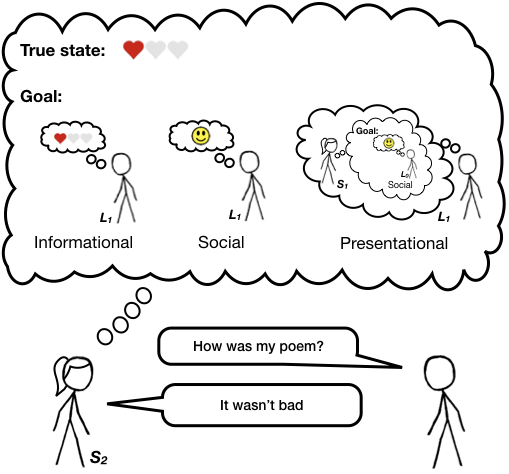
\includegraphics[width=\textwidth]{fig/model} \caption{Diagram of the model: The pragmatic speaker observes the true state and determines her goal between three utilities (informational, social, and presentational), and produces an utterance.}\label{fig:model}
\end{figure}

RSA models are defined recursively such that speakers reason about
listeners, and vice versa. By convention this recursion is indexed such
that a pragmatic listener \(L_1\) reasons about what intended meaning
and goals would have led a speaker \(S_1\) to produce a particular
utterance. Then \(S_1\) reasons about a \enquote{literal listener}
\(L_0\), modeled as attending only to the literal meanings of words
(rather than their pragmatic implications), and hence grounds the
recursion. The target of our current work is a model of a polite speaker
\(S_2\): \(S_2\) reasons about what utterance to say to \(L_1\) by
considering the set of utilities described above (Figure
\ref{fig:model}).

We evaluate our model on its ability to predict human utterance choices
in situations where polite language use is expected. Imagine Bob recited
his poem and asks Ann how well he did. Ann (\(S_2\)) produces an
utterance \(w\) based on the true state of the world \(s\) (i.e., the
rating truly deserved by Bob's recital) and a set of goal weights
\(\hat{\phi}\), that determines how much Ann prioritizes each goal.
Ann's production decision is softmax, which interpolates between
maximizing and probability matching (via \(\lambda_{S_2}\); Goodman \&
Stuhlmüller, 2013):

\[P_{S_2}(w | s, \hat{\phi}) \propto \exp(\lambda_{S_2} \cdot \mathop{\mathbb{E}}[U_{total}(w; s; \hat{\phi})])\].

What goals must the speaker consider to arrive at a polite utterance? We
consider three utilities: informational, social, and presentational. The
total utility of an utterance is the weighted combination of the three
utilities minus the utterance cost \(C(w)\):

\[U_{total}(w; s; \hat{\phi}) = \phi_{inf} \cdot U_{inf}(w; s) + \phi_{soc} \cdot U_{soc}(w; s) + \phi_{pres} \cdot U_{pres}(w; s) - C(w)\].

The first utility term is a standard \emph{informational utility}
(\(U_{inf}\)), which represents the speaker's desire to be epistemically
helpful. The informational utility captures the amount of information a
literal listener (\(L_0\)) would still not know about the world state
\(s\) after hearing the speaker's utterance \(w\) (i.e., surprisal):
\(U_{inf}(w) = \ln(P_{L_1}(s | w))\).

For aspects of the world with affective consequences for the listener
(e.g., Bob and his poem recital), we assume speakers produce utterances
that make listeners feel like they are in a good state. The second
utility term is a \emph{social utility} (\(U_{soc}\)), which we define
as the expected subjective utility \(V(s)\) of the state implied to the
listener by the utterance:
\(U_{soc}(w) = \mathbb{E}_{P_{L_1}(s \mid w)}[V(s)]\). In our
experimental domain, states are explicit ratings, so we use a positive
linear value function \(V\) to capture the idea that listeners want to
hear that they are in a good state of the world (e.g., Bob prefers that
his poem was good).

If listeners try to infer the goals that a speaker is entertaining
(e.g., social vs.~informational), speakers may choose utterances in
order to convey that they had certain goals in mind. The third and the
most novel component of our model, \emph{presentational utility}
(\(U_{pres}\)), captures the extent to which the speaker \emph{appears}
to the listener to have a particular goal in mind (e.g., to be kind).
The speaker gains presentational utility when her listener believes she
has certain goals -- that she is trying to be informative or kind.
Formally,

\[U_{pres}(w) = \ln(P_{L_1}(\phi_{S_1} \mid w)) = \ln \int_s P_{L_1}(s, \phi_{S_1} \mid w)\].

To define this term, the speaker has a weighting of informational
vs.~social goals to convey (\(\phi_{S_1}\)) and must consider the
beliefs of listener L1, who hears an utterance and jointly infers both
the speaker's utilities and the true state of the world:

\[P_{L_1}(s, \hat{\phi} | w) \propto P_{S_1}(w | s, \hat{\phi}) \cdot P(s) \cdot p(\hat{\phi})\].

This presentational utility is higher-order in that it can only be
defined for a speaker thinking about a listener who evaluates a speaker
(i.e., it can be defined for \(S_2\), but not \(S_1\)).

Finally, more complex utterances incur a greater cost, \(C(w)\) --
capturing the general pressure towards economy in speech. In our work,
utterances with negation (e.g., \enquote{not terrible}) are assumed to
be slightly costlier than their equivalents with no negation (inferred
from data; see Supplementary Information).

Within our experimental domain, we assume there are four possible states
of the world corresponding to the value placed on a particular referent
(e.g., the presentation the speaker is commenting on):
\(S = {s_1,...,s_5}\). We further assume a uniform prior distribution
over possible states of the world. The set of utterances is
\{\emph{terrible}, \emph{bad}, \emph{good}, \emph{amazing}, \emph{not
terrible}, \emph{not bad}, \emph{not good}, and \emph{not amazing}\}. We
implemented this model using the probabilistic programming language
WebPPL (Goodman \& Stuhlmüller, 2014).

Intuitively, if Bob's performance was good, Ann's utilities align toward
a positive utterance. By saying \enquote{{[}Your poem{]} was amazing,}
Ann is simultaneously being truthful, kind, and appearing both truthful
and kind. If Bob's performance was poor, however, Ann is in a bind: Ann
could be kind and say \enquote{It was great}, but at the cost of
conveying the wrong information to Bob if he believes her to be
truthful. If he does not, he might infer Ann is \enquote{just being
nice}, but is uninformative. Alternatively, she could say the truth
(\enquote{It was bad}), but then Bob would think Ann didn't care about
him. What is a socially-aware speaker to do? Our model predicts that
indirect speech -- like \enquote{It wasn't bad} -- helps navigate Ann's
dilemma. Her statement is sufficiently vague to leave open the
possibility that the poem was good, but her avoidance of the simpler and
less costly \enquote{It was good} provides both an inference that the
performance was mediocre and a signal that she cares about Bob's
feelings.

We made a direct, pre-registered test of our model by instantiating the
example above in an online experiment (\emph{N} = 202). Participants
read scenarios in which we provided information on the speaker's (Ann's,
in our example) feelings toward some performance or product (e.g., poem
recital; \emph{true state}), on a scale from zero to three hearts (e.g.,
one out of three hearts). For example, one trial read: \enquote{Imagine
that Bob gave a poem recital, but he didn't know how good it was. Bob
approached Ann, who knows a lot about poems, and asked}How was my poem?"
We also manipulated the speaker's \emph{goal} across trials: to be
\emph{informative} (\enquote{give accurate and informative feedback});
to be \emph{kind} (\enquote{make the listener feel good}); or to be
\emph{both} informative and kind simultaneously. We hypothesized that
each of the three goals will represent a tradeoff between the three
utilities in our model (see Supplementary Information). In a single
trial, each scenario was followed by a question asking for the most
likely utterance by Ann. Participants selected one of eight possible
utterances, by choosing between \emph{It was} vs. \emph{It wasn't} and
then among \emph{terrible}, \emph{bad}, \emph{good}, and \emph{amazing.}

\begin{figure}[!h]
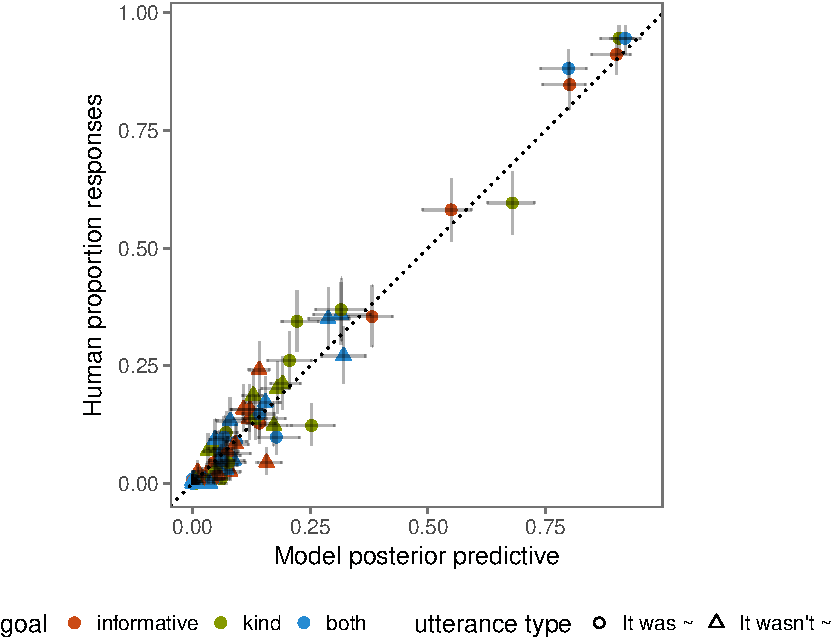
\includegraphics[width=\textwidth]{polite_NHB_files/figure-latex/variance-1} \caption{Full distribution of human responses vs. model predictions. Error bars represent 95\% confidence intervals for the data (vertical) and 95\% highest density intervals for the model (horizontal).}\label{fig:variance}
\end{figure}

Our primary behavioral hypothesis was that speakers describing bad
states (e.g., Bob's performance deserved 0 heart) with goals to be both
informative and kind would produce more indirect, negative utterances
(e.g., \enquote{It wasn't terrible}). Such indirect speech acts serve to
save the listener's face while also conveying a vague estimate of the
true state. This prediction was confirmed: a Bayesian mixed-effects
model predicting negation as a function of true state and goal yielded
an interaction such that a speaker with both goals to be informative and
kind produced more negation in worse states compared to a speaker with
only the goal to be informative (\emph{M} = -1.33, {[}-1.69, -0.98{]})
and goal to be kind (\emph{M} = -0.50, {[}-0.92, -0.07{]}). Rather than
eschewing one of their goals to increase utility along a single
dimension, participants chose utterances that jointly satisfied their
conflicting goals by producing indirect, polite speech.

\begin{figure}[!h]
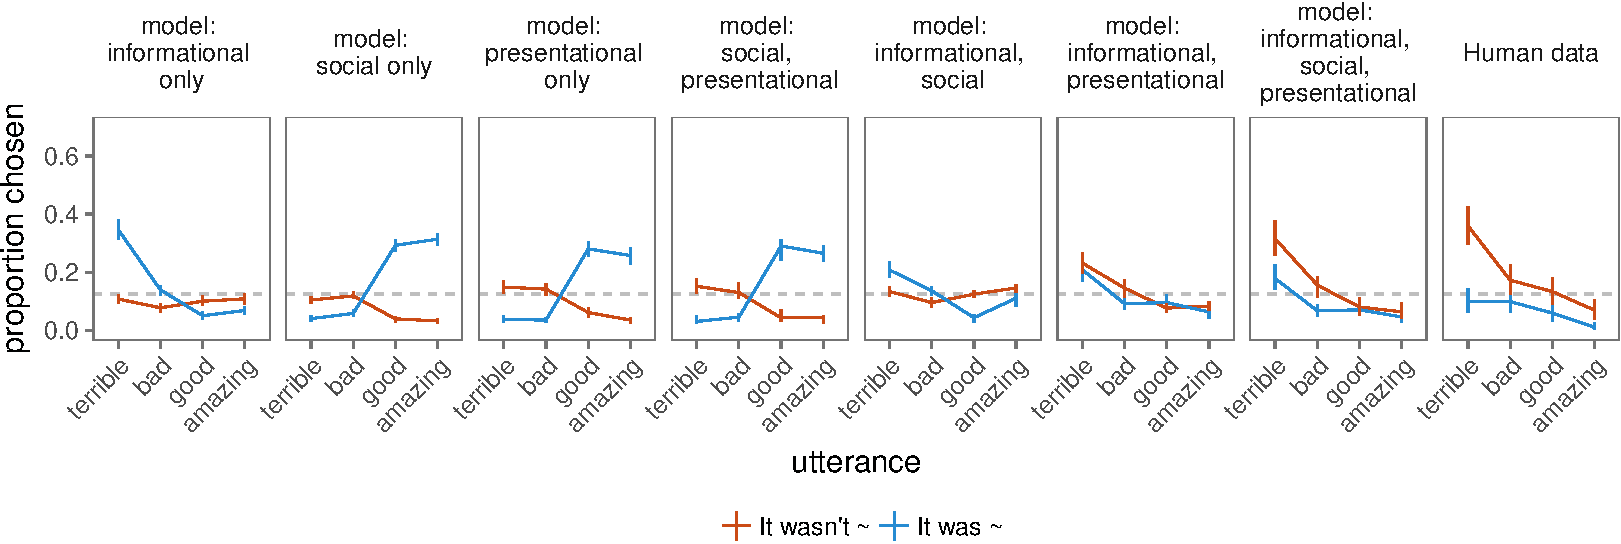
\includegraphics[width=\textwidth]{polite_NHB_files/figure-latex/comparison-1} \caption{Comparison of predictions for proportion of utterances chosen by pragmatic speaker from possible model variants (left) and human data (rightmost) for average proportion of negation produced among all utterances, given true state of 0 heart (on a scale of 0 to 3) and speaker with both goals to be informative and kind. Gray dotted line indicates chance level at 12.5\%.}\label{fig:comparison}
\end{figure}

\begin{table}[tbp]
\begin{center}
\begin{threeparttable}
\caption{\label{tab:comparisonTable}Comparison of variance explained for each model variant and log Bayes Factors quantifying evidence in favor of alternative model in comparison.}
\begin{tabular}{lll}
\toprule
Model & \multicolumn{1}{c}{Variance 
explained} & \multicolumn{1}{c}{log BF}\\
\midrule
model: 
informational, 
social, 
presentational & 0.97 & --\\
model: 
informational, 
presentational & 0.96 & -11.14\\
model: 
informational, 
social & 0.92 & -25.06\\
model: 
social, 
presentational & 0.23 & -864\\
model: 
presentational 
only & 0.23 & -873.83\\
model: 
social only & 0.22 & -885.52\\
model: 
informational 
only & 0.83 & -274.89\\
\bottomrule
\end{tabular}
\end{threeparttable}
\end{center}
\end{table}

Next, to connect the behavioral data to our model, we inferred the
parameters of the RSA model (e.g., the speaker's utility weights in each
goal condition; see Supplementary Information) via a Bayesian data
analysis (M. D. Lee \& Wagenmakers, 2014). To approximate the semantics
of the words as interpreted by the literal listener \(L_0\), we obtained
literal meaning judgments from an independent group of participants
(\emph{N}=51). Predictions from the full polite speaker model showed a
very strong fit to participants' utterance choices (\(r^2\)(96) = 0.97;
Figure \ref{fig:variance}).

We also compared the predictions of our model to its variants containing
subsets of the three utilities in the full model. Both the variance
explained and the marginal likelihood of the observed data were the
highest for the full model (Table \ref{tab:comparisonTable}). Only the
full model captured the participants' preference for negation in the
condition in which the speaker had both goals to be informative and kind
about truly bad states, as hypothesized (Figure \ref{fig:comparison}).
All three utilities -- informational, social, and presentational -- were
required to fully explain participants' utterance choices. The utility
weights inferred for the full model (Table \ref{tab:phi}) provide
additional insight into how polite language use operates: our condition
manipulation altered the balance between these weights, but all
utilities played a role in all conditions.

Politeness is a puzzle for purely informational accounts of language
use. Incorporating social motivations can provide an explanatory
framework, but such intuitions have been resistant to formalization or
precise testing. To overcome this issue, we created a utility-theoretic
model of language use that captured the interplay between competing
informational, social, and presentational goals. A preregistered
experimental test of the model confirmed its ability to capture human
judgments, unlike comparison models that used only a subset of the full
utility structure.

To precisely estimate choice behavior, our experiment abstracted away
from natural interactions in a number of ways. Real speakers have access
to a potentially infinite range of utterances to manage the tradeoffs in
our experiment (\enquote{It's hard to write a good poem}, \enquote{That
metaphor in the second stanza was so relatable!}). Under our framework,
each utterance will have strengths and weaknesses relative to the
speaker's goals, though computation in an unbounded model presents
technical challenges (perhaps paralleling the difficulty human speakers
feel in finding the right thing to say in a difficult situation; see
Goodman \& Frank, 2016).

For a socially-conscious speaker, managing listeners' inferences is a
fundamental task. Inspired by the theory of politeness as face
management (Brown \& Levinson, 1987), our model takes a step towards
understanding it. Our work extends previous models of language beyond
standard informational utilities to address social and
self-presentational concerns. Previous theories of language use have not
explained how informational versus social concerns trade off to inform
the speaker's utterance choices. Thus, this work represents a key
theoretical advance exploring how informational cooperativity interacts
with other social goals. By considering utility-driven inferences in a
social context (Baker, Jara-Ettinger, Saxe, \& Tenenbaum, 2017; Hamlin,
Ullman, Tenenbaum, Goodman, \& Baker, 2013) where agents need to take
into account concerns about both self and others, our approach here
could give insights into a wide range of social behaviors beyond speech.

The model presented here relates to other work done in game-theoretic
pragmatics. Van Rooy (2003) uses a game-theoretic analysis of polite
requests (\enquote{Could you possibly take me home?}) to argue the
purpose of polite language is to align the preferences of interlocutors.
Our notion of social utility \(U_{soc}\) and presentational utility
\(U_{pres}\) is similar in that they motivate speakers to signal worlds
that make the listener feel good. Van Rooy (2003)'s analysis, however,
relies on the notion that polite language is costly (in a social way
e.g., by reducing one's social status or incurring social debt to one's
conversational partner) but it's not clear how the polite behaviors
explored in our experiments (not polite requests) would incur any cost
to speaker or listener. Our model derives its predictions by construing
the speaker utility as a collection of possible goals (here, epistemic,
social, and presentational goals). The speech-acts themselves are not
costly. In Pinker, Nowak, and Lee (2008)'s model, human communication is
assumed to involve a mixture of cooperation \emph{and} conflict:
indirect speech then allows for plausible deniability that is in
self-interest but goes against the interest of the addressee. In
contrast, our work builds on existing classic theories of polite speech
as primarily cooperative (Brown \& Levinson, 1987; Grice, 1975) rather
than based on both cooperation and conflict. We have shown that a
separate notion of plausible deniability may not be needed, as indirect
speech in our specific case comes from both a goal to be helpful and a
desire to look good. Our work is able to capture different linguistic
nuances involved in this process of reasoning about different goals that
speakers have.

By experimenting with different utility weights and value functions, our
model could provide a framework for understanding systematic
cross-cultural differences in what counts as polite. For example,
following Brown and Levinson (1987), cross-cultural differences in
politeness could be a product of different weightings within the same
utility structure. It is also possible, however, that culture affects
the value function \(V\) that maps states of the world onto subjective
values for the listener (e.g., the mapping from states to utilities may
be more complex than we have considered). Our formal modeling approach
with systematic behavior measurements provides an avenue towards
understanding the vast range of politeness practices found across
languages.

Politeness is only one of the ways that language use deviates from pure
information transfer. When we flirt, insult, boast, and empathize, we
also balance being informative with goals to affect others' feelings and
present particular views of ourselves. Our work shows how social and
self-presentational motives can be integrated with other concerns more
generally, opening up the possibility for a broader theory of social
language. Further, a formal account of politeness moves us closer to
courteous computation -- to computers that can communicate with tact.

\section{Acknowledgments}\label{acknowledgments}

This work was supported by NSERC PGS Doctoral scholarship
PGSD3-454094-2014 to EJY, NSF Graduate Research Fellowship DGE-114747 to
MHT, ONR grant N00014-13-1-0788 to NDG, and NSF grant BCS 1456077 to
MCF.

\newpage

\section{Methods}\label{methods}

\subsection{Literal semantic task}\label{literal-semantic-task}

We probed judgments of literal meanings of the target words assumed by
our model and used in our main experiment. 51 participants with IP
addresses in the United States were recruited on Amazon's Mechanical
Turk. We used thirteen different context items in which a speaker
evaluated a performance of some kind. For example, in one of the
contexts, Ann saw a presentation, and Ann's feelings toward the
presentation (true state) were shown on a scale from zero to three
hearts (e.g., two out of three hearts filled in red color; see
Figure~\ref{fig:screenshot} for an example of the heart scale). The
question of interest was \enquote{Do you think Ann thought the
presentation was / wasn't X?} and participants responded by choosing
either \enquote{no} or \enquote{yes.} The target could be one of four
possible words: \emph{terrible}, \emph{bad}, \emph{good}, and
\emph{amazing}, giving rise to eight different possible utterances (with
negation or no negation). Each participant read 32 scenarios, depicting
every possible combination of states and utterances. The order of
context items was randomized, and there were a maximum of four repeats
of each context item per participant. For this and the speaker
production experiment, we analyzed the data by collapsing across context
items. For each utterance-state pair, we computed the posterior
distribution over the semantic weight (i.e., how consistent X utterance
is with Y state) assuming a uniform prior over the weight (i.e., a
standard Beta-Binomial model). Meanings of the words as judged by
participants were as one would expect (Figure ~\ref{fig:litsem}).

\begin{figure}[!h]
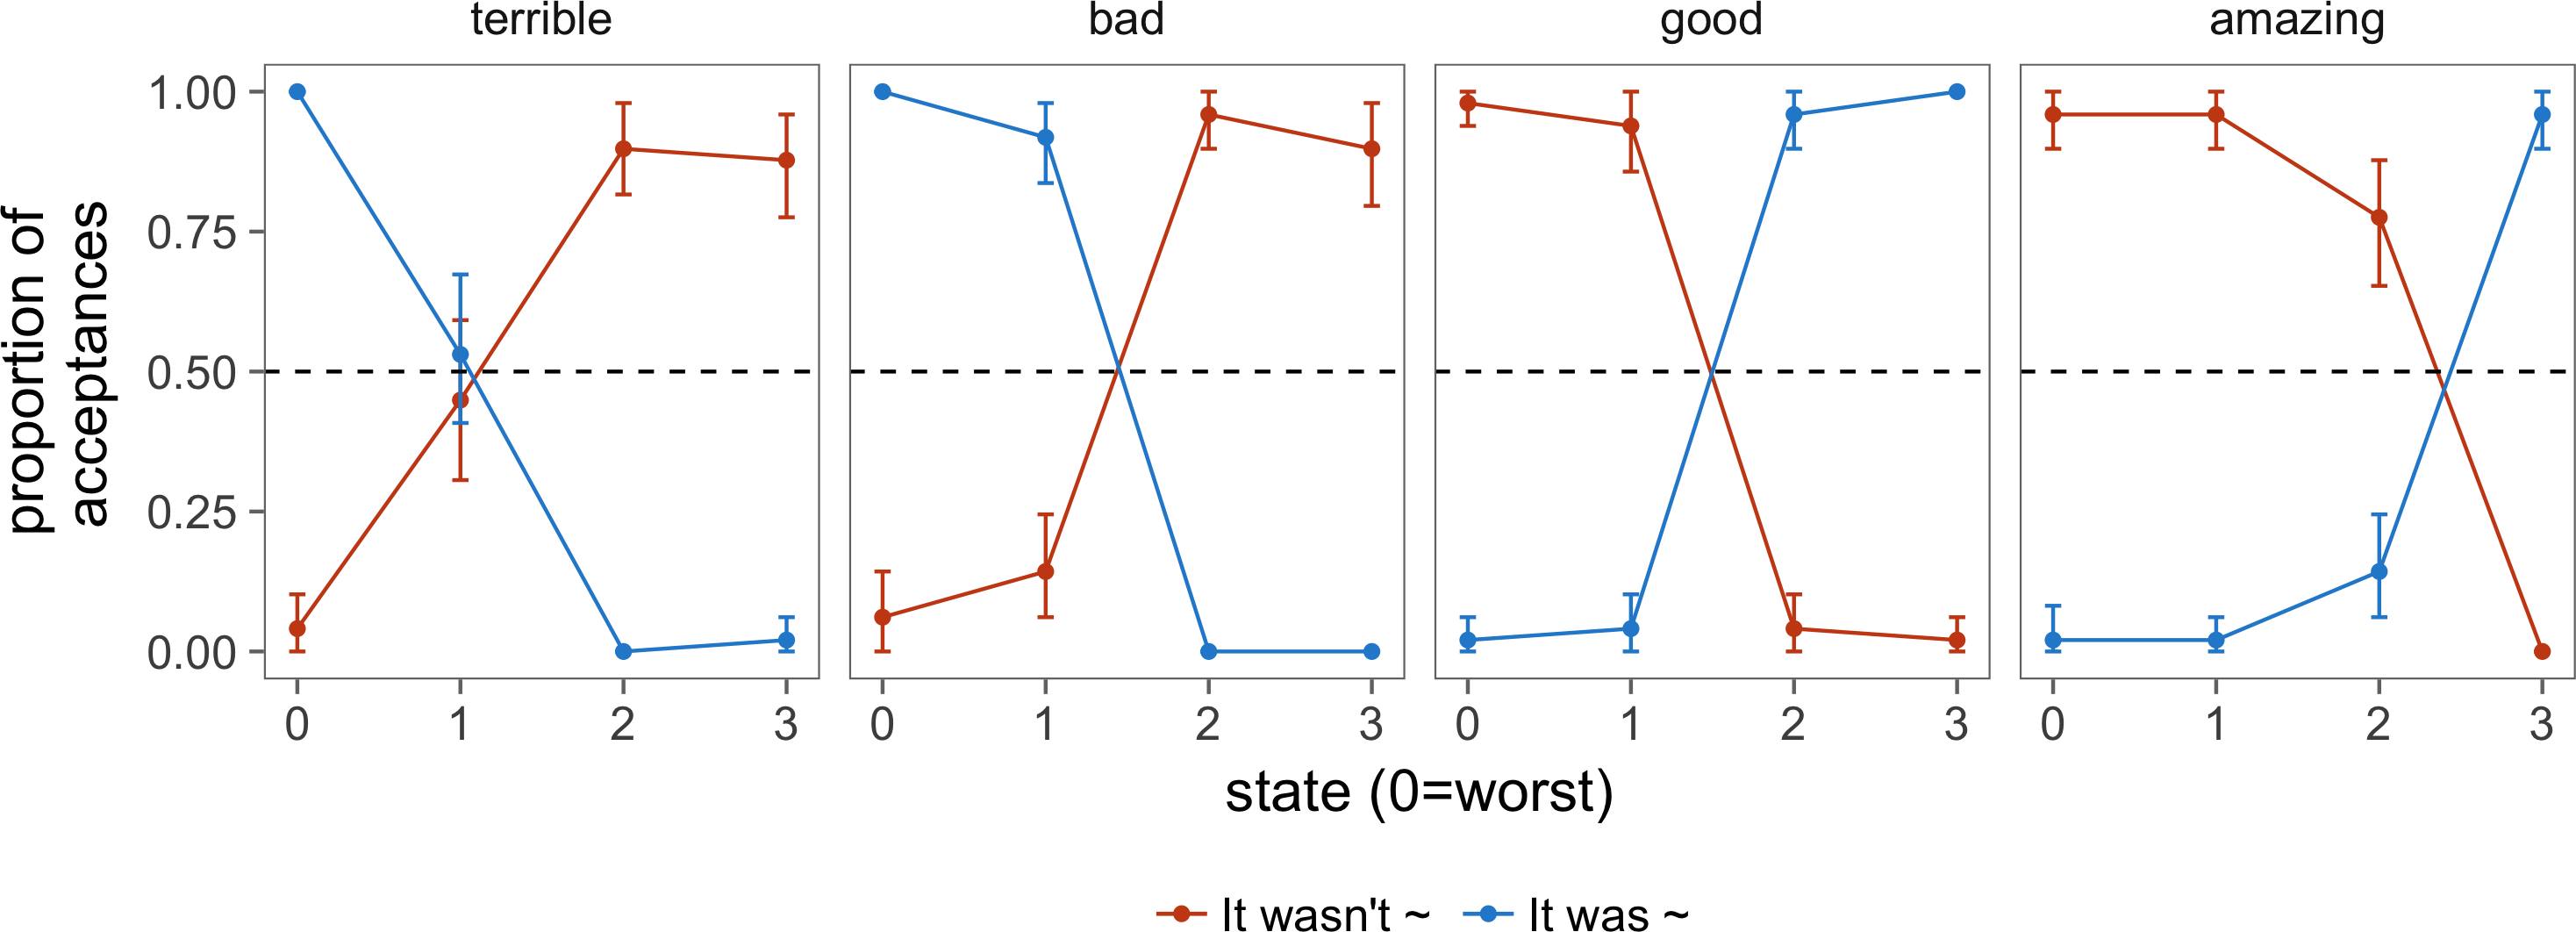
\includegraphics[width=\textwidth]{polite_NHB_files/figure-latex/litsem-1} \caption{Semantic measurement results. Proportion of acceptances of utterance types (shown in different colors) combined with target words (shown in different facets) given the true state represented on a scale of hearts. Error bars represent 95\% confidence intervals.}\label{fig:litsem}
\end{figure}

\subsection{Speaker production task}\label{speaker-production-task}

\begin{figure}[!h]
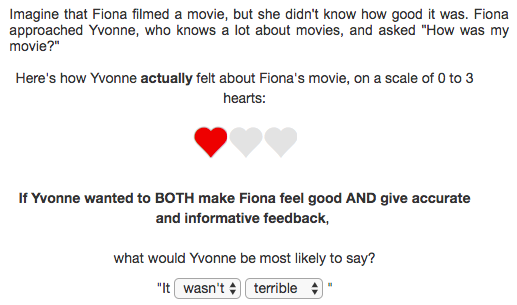
\includegraphics[width=\textwidth]{fig/screenshot} \caption{Example of a trial in the speaker production task.}\label{fig:screenshot}
\end{figure}

202 participants with IP addresses in the United States were recruited
on Amazon's Mechanical Turk. As in the literal semantic task above, we
used scenarios in which a person (e.g., Bob) gave some performance and
asked for another person (e.g., Ann)'s opinion on the performance
(Figure ~\ref{fig:screenshot}). Additionally, we provided information on
the speaker Ann's goal -- to make Bob feel good, or to give as accurate
and informative feedback as possible, or both -- and the true state --
how Ann actually felt about Bob's performance (e.g., two out of three
hearts, on a scale from zero to three hearts;
Figure~\ref{fig:screenshot}). Each participant read twelve scenarios,
depicting every possible combination of the three goals and four states.
The order of context items was randomized, and there were a maximum of
two repeats of each context item per participant. Each scenario was
followed by a question that read, \enquote{If Ann wanted to make Bob
feel good but not necessarily give informative feedback (or to give
accurate and informative feedback but not necessarily make Bob feel
good, or BOTH make Bob feel good AND give accurate and informative
feedback), what would Ann be most likely to say?} Participants indicated
their answer by choosing one of the options on the two dropdown menus,
side-by-side, one for choosing between \emph{It was} vs. \emph{It
wasn't} and the other for choosing among \emph{terrible}, \emph{bad},
\emph{good}, and \emph{amazing.}

\subsection{Data availability}\label{data-availability}

Our model, preregistration of hypotheses, procedure, data, and analyses
are available at \url{https://github.com/ejyoon/polite_speaker}.

\section{Author information}\label{author-information}

\subsection{Author contributions}\label{author-contributions}

All authors designed research and wrote the paper; E.J.Y. and M.H.T.
performed research and analyzed data.

\subsection{Competing interests}\label{competing-interests}

The authors declare no conflict of interest.

\section{Supplementary Information}\label{supplementary-information}

\subsection{Data analysis}\label{data-analysis}

We used R (Version 3.4.3; R Core Team, 2017) and the R-packages
\emph{BayesFactor} (Version 0.9.12.2; Morey \& Rouder, 2015),
\emph{bindrcpp} (Version 0.2; Müller, 2017a), \emph{binom} (Version
1.1.1; Dorai-Raj, 2014), \emph{brms} (Version 2.0.1; Bürkner, 2017),
\emph{coda} (Version 0.19.1; Plummer, Best, Cowles, \& Vines, 2006),
\emph{directlabels} (Version 2017.3.31; Hocking, 2017), \emph{dplyr}
(Version 0.7.4; Wickham, Francois, Henry, \& Müller, 2017),
\emph{forcats} (Version 0.2.0; Wickham, 2017a), \emph{ggplot2} (Version
2.2.1; Wickham, 2009), \emph{ggthemes} (Version 3.4.0; Arnold, 2017),
\emph{gridExtra} (Version 2.3; Auguie, 2017), \emph{here} (Version 0.1;
Müller, 2017b), \emph{jsonlite} (Version 1.5; Ooms, 2014),
\emph{langcog} (Version 0.1.9001; Braginsky, Yurovsky, \& Frank, n.d.),
\emph{lme4} (Version 1.1.15; Bates, Mächler, Bolker, \& Walker, 2015),
\emph{magrittr} (Version 1.5; Bache \& Wickham, 2014), \emph{Matrix}
(Version 1.2.12; Bates \& Maechler, 2017), \emph{papaja} (Version
0.1.0.9655; Aust \& Barth, 2017), \emph{purrr} (Version 0.2.4; Henry \&
Wickham, 2017), \emph{RColorBrewer} (Version 1.1.2; Neuwirth, 2014),
\emph{Rcpp} (Eddelbuettel \& Balamuta, 2017; Version 0.12.17;
Eddelbuettel \& François, 2011), \emph{readr} (Version 1.1.1; Wickham,
Hester, \& Francois, 2017), \emph{rwebppl} (Version 0.1.97; Braginsky,
Tessler, \& Hawkins, n.d.), \emph{stringr} (Version 1.3.1; Wickham,
2017b), \emph{tibble} (Version 1.4.2; Müller \& Wickham, 2017),
\emph{tidyr} (Version 0.7.2; Wickham \& Henry, 2017), and
\emph{tidyverse} (Version 1.2.1; Wickham, 2017c) for all our analyses.

\subsection{Full statistics on human
data}\label{full-statistics-on-human-data}

\begin{table}[tbp]
\begin{center}
\begin{threeparttable}
\caption{\label{tab:brmTab}Predictor mean estimates with standard deviation and 95\% credible interval information for a Bayesian linear mixed-effects model predicting negation production based on true state and speaker goal (with both-goal as the reference level).}
\begin{tabular}{lllll}
\toprule
Predictor & \multicolumn{1}{c}{Mean} & \multicolumn{1}{c}{SD} & \multicolumn{1}{c}{95\% CI-Lower} & \multicolumn{1}{c}{95\% CI-Upper}\\
\midrule
Intercept & 0.88 & 0.13 & 0.63 & 1.12\\
True state & 2.18 & 0.17 & 1.86 & 2.53\\
Goal: Informative & 0.47 & 0.17 & 0.14 & 0.80\\
Goal: Kind & 0.97 & 0.25 & 0.51 & 1.49\\
True state * Informative & -1.33 & 0.18 & -1.69 & -0.98\\
True state * Kind & -0.50 & 0.22 & -0.92 & -0.07\\
\bottomrule
\end{tabular}
\end{threeparttable}
\end{center}
\end{table}

We used Bayesian linear mixed-effects models (\texttt{brms} package in
R; Bürkner, 2017) using crossed random effects of true state and goal
with maximal random effects structure (Barr, Levy, Scheepers, \& Tily,
2013; Gelman \& Hill, 2006).

\subsection{Model fitting and inferred
parameters}\label{model-fitting-and-inferred-parameters}

\begin{table}[tbp]
\begin{center}
\begin{threeparttable}
\caption{\label{tab:phi}Inferred phi parameters from all model variants with more than one utility.}
\begin{tabular}{llllll}
\toprule
Model & \multicolumn{1}{c}{goal} & \multicolumn{1}{c}{$\phi_{inf}$} & \multicolumn{1}{c}{$\phi_{soc}$} & \multicolumn{1}{c}{$\phi_{pres}$} & \multicolumn{1}{c}{$\phi_{S_1}$}\\
\midrule
informational, social, presentational & both & 0.36 & 0.11 & 0.54 & 0.36\\
informational, social, presentational & informative & 0.36 & 0.02 & 0.62 & 0.49\\
informational, social, presentational & social & 0.25 & 0.31 & 0.44 & 0.37\\
informational, presentational & both & 0.64 & NA & 0.36 & 0.17\\
informational, presentational & informative & 0.77 & NA & 0.23 & 0.33\\
informational, presentational & social & 0.66 & NA & 0.34 & 0.04\\
informational, social & both & 0.54 & 0.46 & NA & NA\\
informational, social & informative & 0.82 & 0.18 & NA & NA\\
informational, social & social & 0.39 & 0.61 & NA & NA\\
social, presentational & both & NA & 0.38 & 0.62 & 0.55\\
social, presentational & informative & NA & 0.35 & 0.65 & 0.75\\
social, presentational & social & NA & 0.48 & 0.52 & 0.66\\
\bottomrule
\end{tabular}
\end{threeparttable}
\end{center}
\end{table}

\begin{table}[tbp]
\begin{center}
\begin{threeparttable}
\caption{\label{tab:otherParams}Inferred negation cost and speaker optimality parameters for all model variants.}
\begin{tabular}{lll}
\toprule
Model & \multicolumn{1}{c}{Cost of negation} & \multicolumn{1}{c}{Speaker optimality}\\
\midrule
informational only & 1.58 & 8.58\\
informational, presentational & 1.89 & 2.93\\
informational, social & 1.11 & 3.07\\
informational, social, presentational & 2.64 & 4.47\\
presentational only & 2.58 & 9.58\\
social only & 1.73 & 7.23\\
social, presentational & 2.49 & 5.29\\
\bottomrule
\end{tabular}
\end{threeparttable}
\end{center}
\end{table}

In the speaker production task, participants were told the speakers'
intentions (e.g., wanted to make Bob feel good). We assume that the
intention descriptions conveyed some mixture of weights \(\phi_{epi}\),
\(\phi_{soc}\), \(\phi_{pres}\), and \(\phi_{S_1}\) that the speaker was
using. We put uninformative priors on the unnormalized mixture weights
(\(\phi\) \textasciitilde{} \(Uniform(0,1)\)) separately for each goal
condition (\enquote{wanted to be X}; \emph{kind}, \emph{informative}, or
\emph{both}). In addition, the full model has two global parameters: the
speaker's soft-max parameter \(\lambda_{S_2}\) and soft-max paramater of
the hypothetical speaker that the pragmatic listener reasons about
\(\lambda_{S_1}\). \(\lambda_{S_1}\) was 1, and \(\lambda_{S_2}\) was
inferred from the data: We put a prior that was consistent with those
used for similar models in this model class: \(\lambda_{S_2}\)
\textasciitilde{} \(Uniform(0,20)\). Finally, we incorporate the literal
semantics data into the RSA model by maintaining uncertainty about the
semantic weight of utterance \(w\) for state \(s\), for each of the
states and utterances, and assuming a Beta-Binomial linking function
between these weights and the literal semantics data (see \emph{Literal
semantics task} above). We infer the posterior distribution over all of
the model parameters and generate model predictions based on this
posterior distribution using Bayesian data analysis (M. D. Lee \&
Wagenmakers, 2014). We ran 4 MCMC chains for 80,000 iterations,
discarding the first 40,000 for burnin. The inferred values of weight
mixtures for each model variant (with different \(\phi\) components) and
other parameters are shown in Table \ref{tab:phi} and Table
\ref{tab:otherParams}, respectively.

\newpage

\subsection{Supplemental Figures}\label{supplemental-figures}

\begin{figure}[!h]
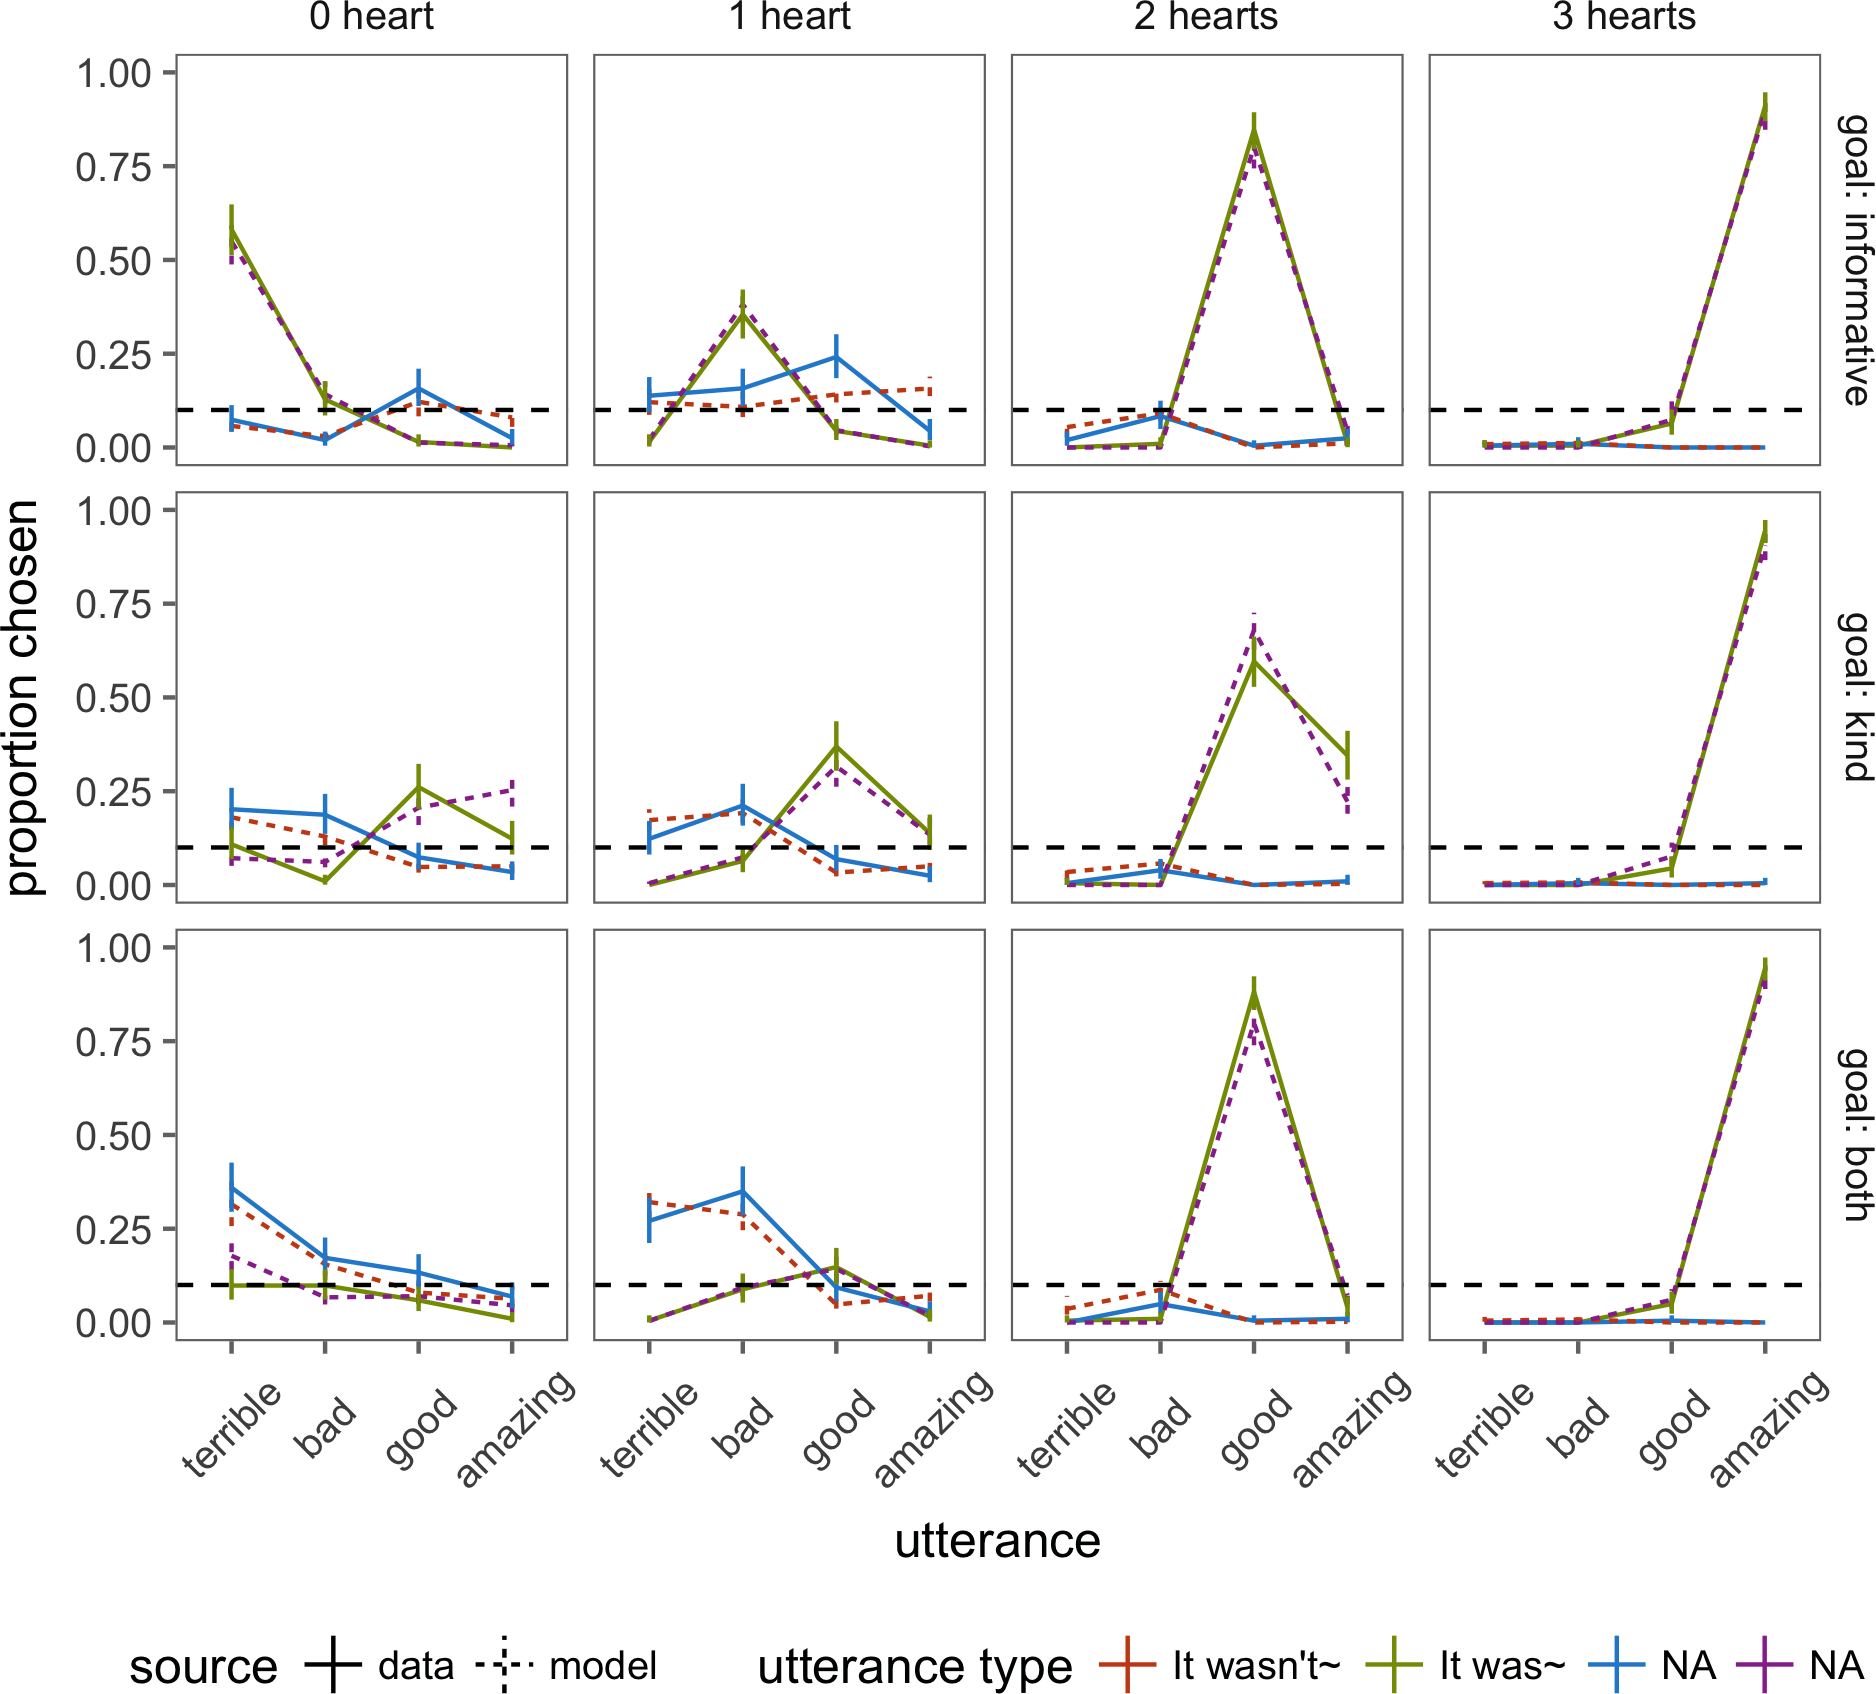
\includegraphics[width=\textwidth]{polite_NHB_files/figure-latex/utterance-1} \caption{Experimental results (solid lines) and fitted predictions from the full model (dashed lines) for speaker production. Proportion of utterances chosen (utterance type – direct vs. indirect – in different colors and words shown on x-axis) given the true states (columns) and speaker goals (rows). Error bars represent 95\% confidence intervals for the data and 95\% highest density intervals for the model. Black dotted line represents the chance level.}\label{fig:utterance}
\end{figure}

\begin{figure}[!h]
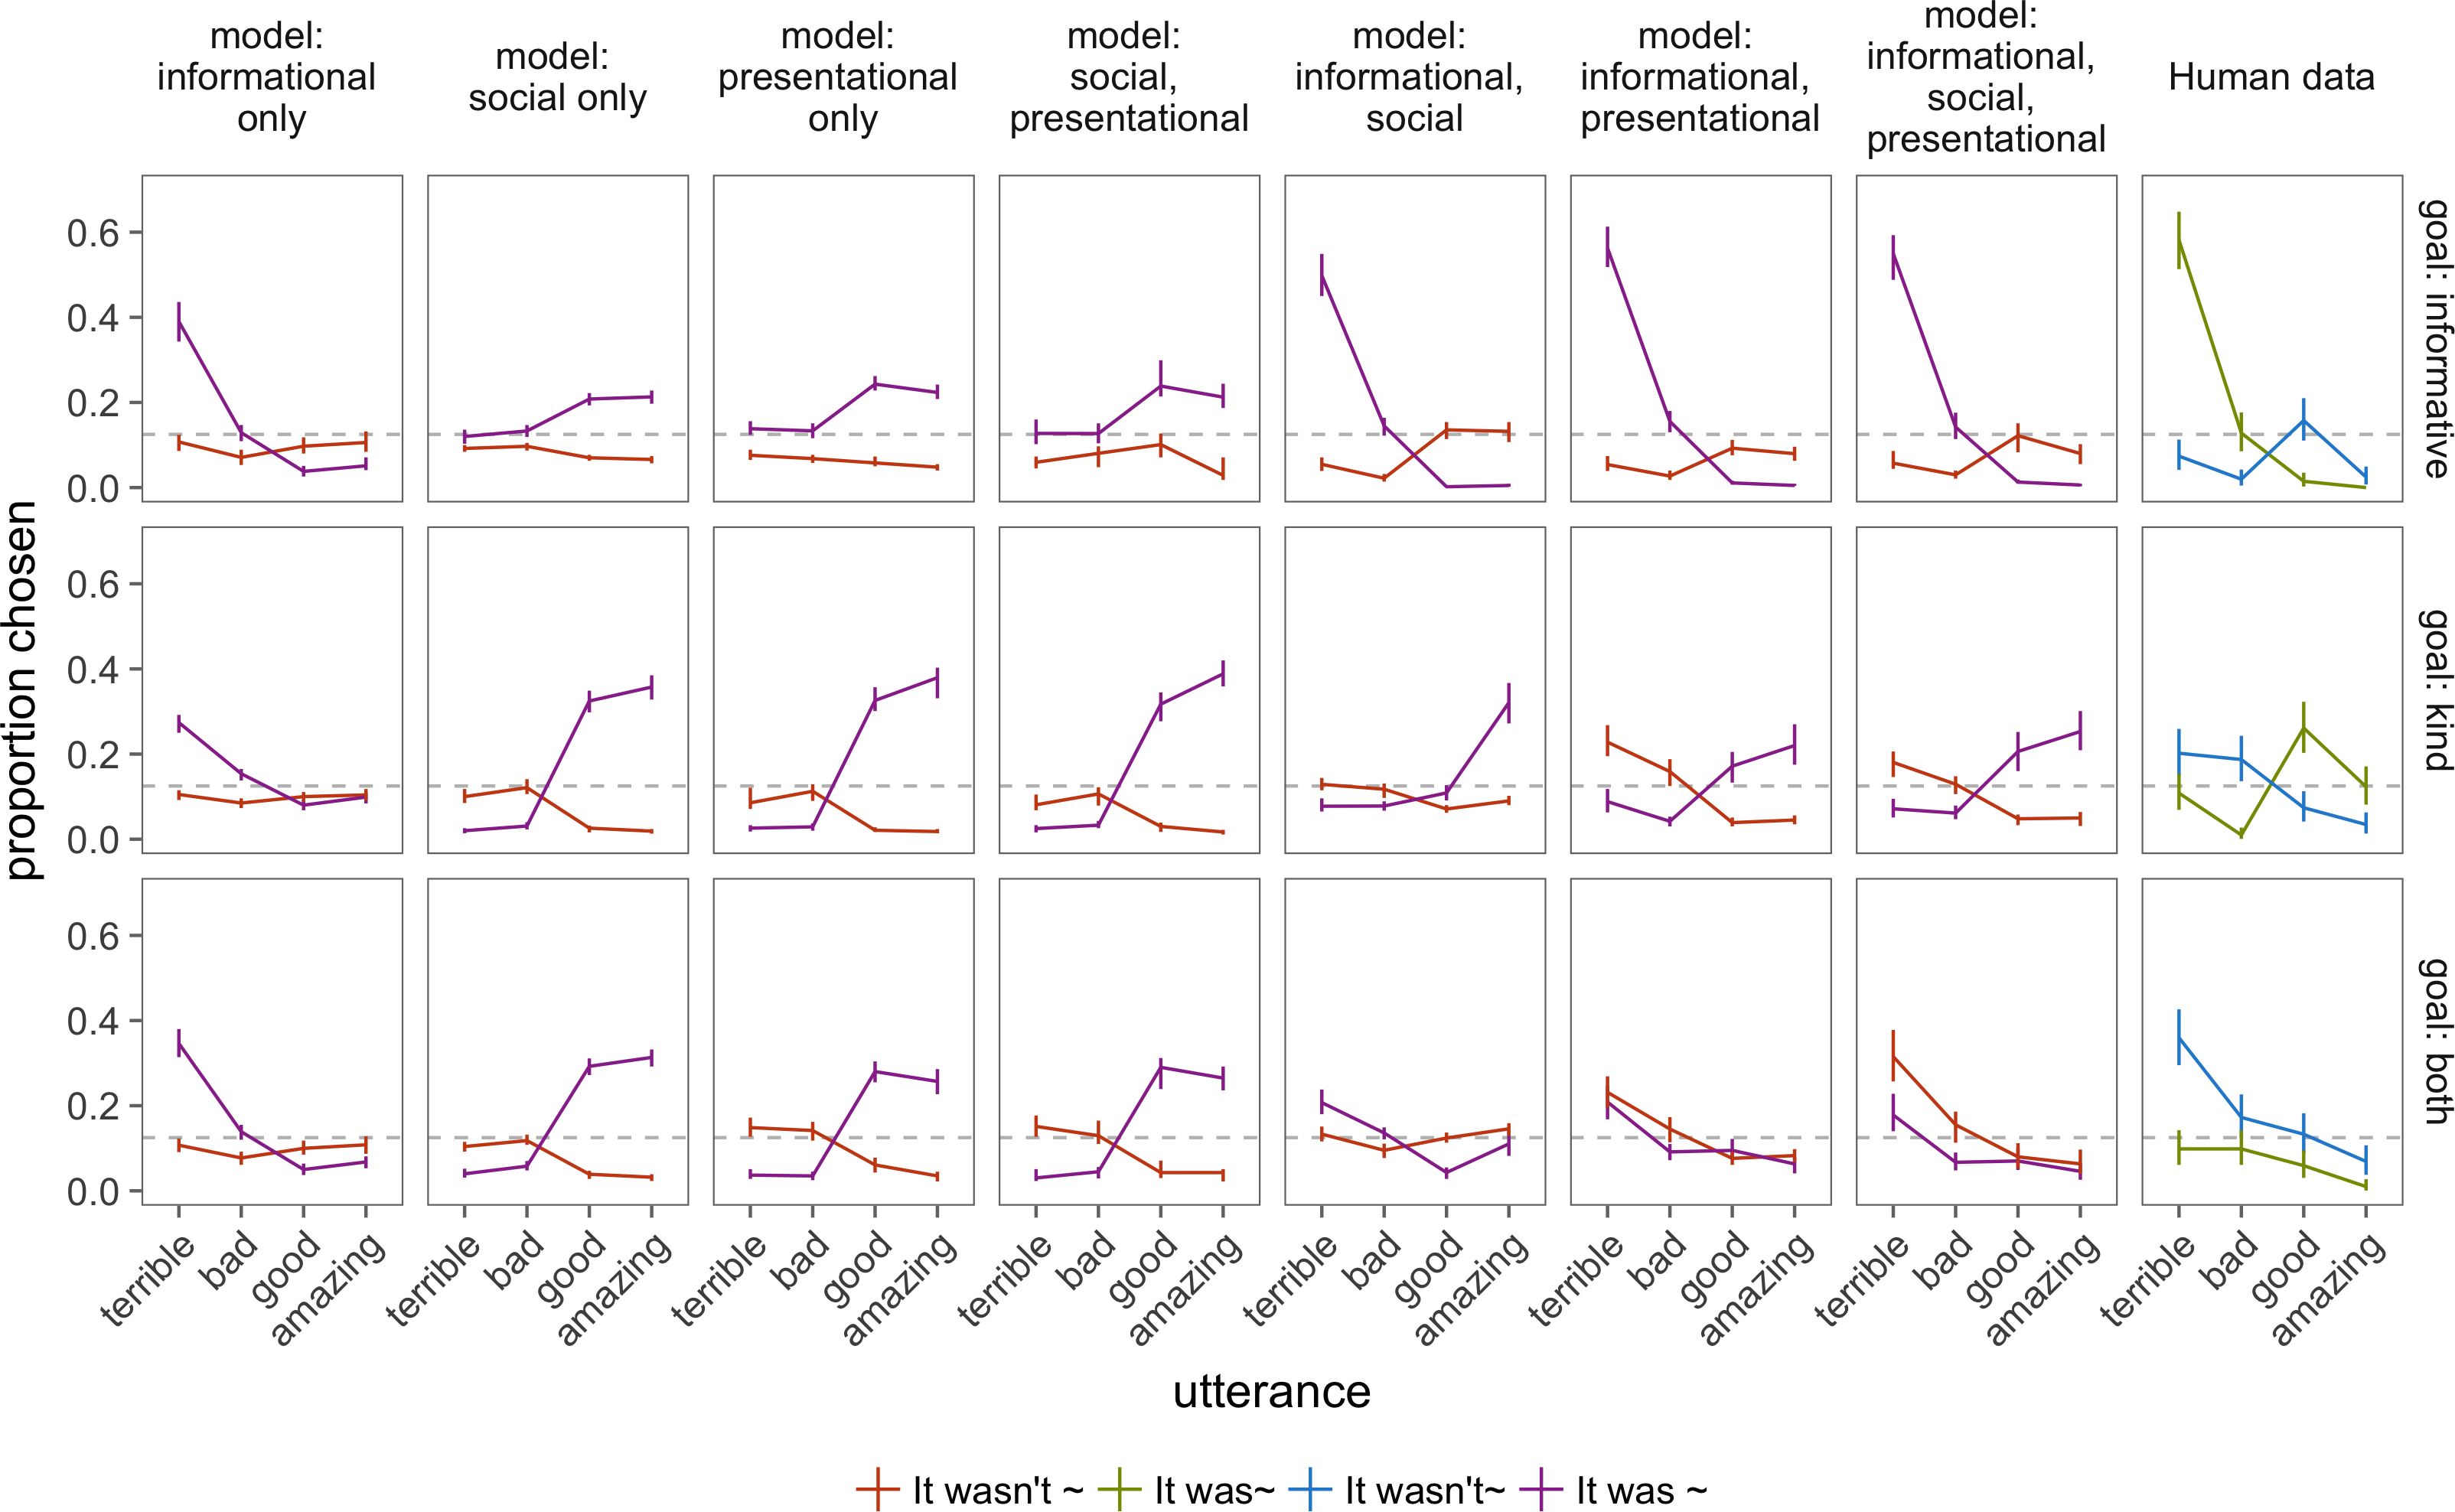
\includegraphics[width=\textwidth]{polite_NHB_files/figure-latex/comparisonAll-1} \caption{Comparison of predictions for proportion of utterances chosen by pragmatic speaker from possible model variants (left) and human data (rightmost) for average proportion of negation produced among all utterances, given true state of 0 heart and speaker with a goal to be informative (top), kind (middle), or both (bottom). Gray dotted line indicates chance level at 12.5\%.}\label{fig:comparisonAll}
\end{figure}

\begin{figure}[!h]
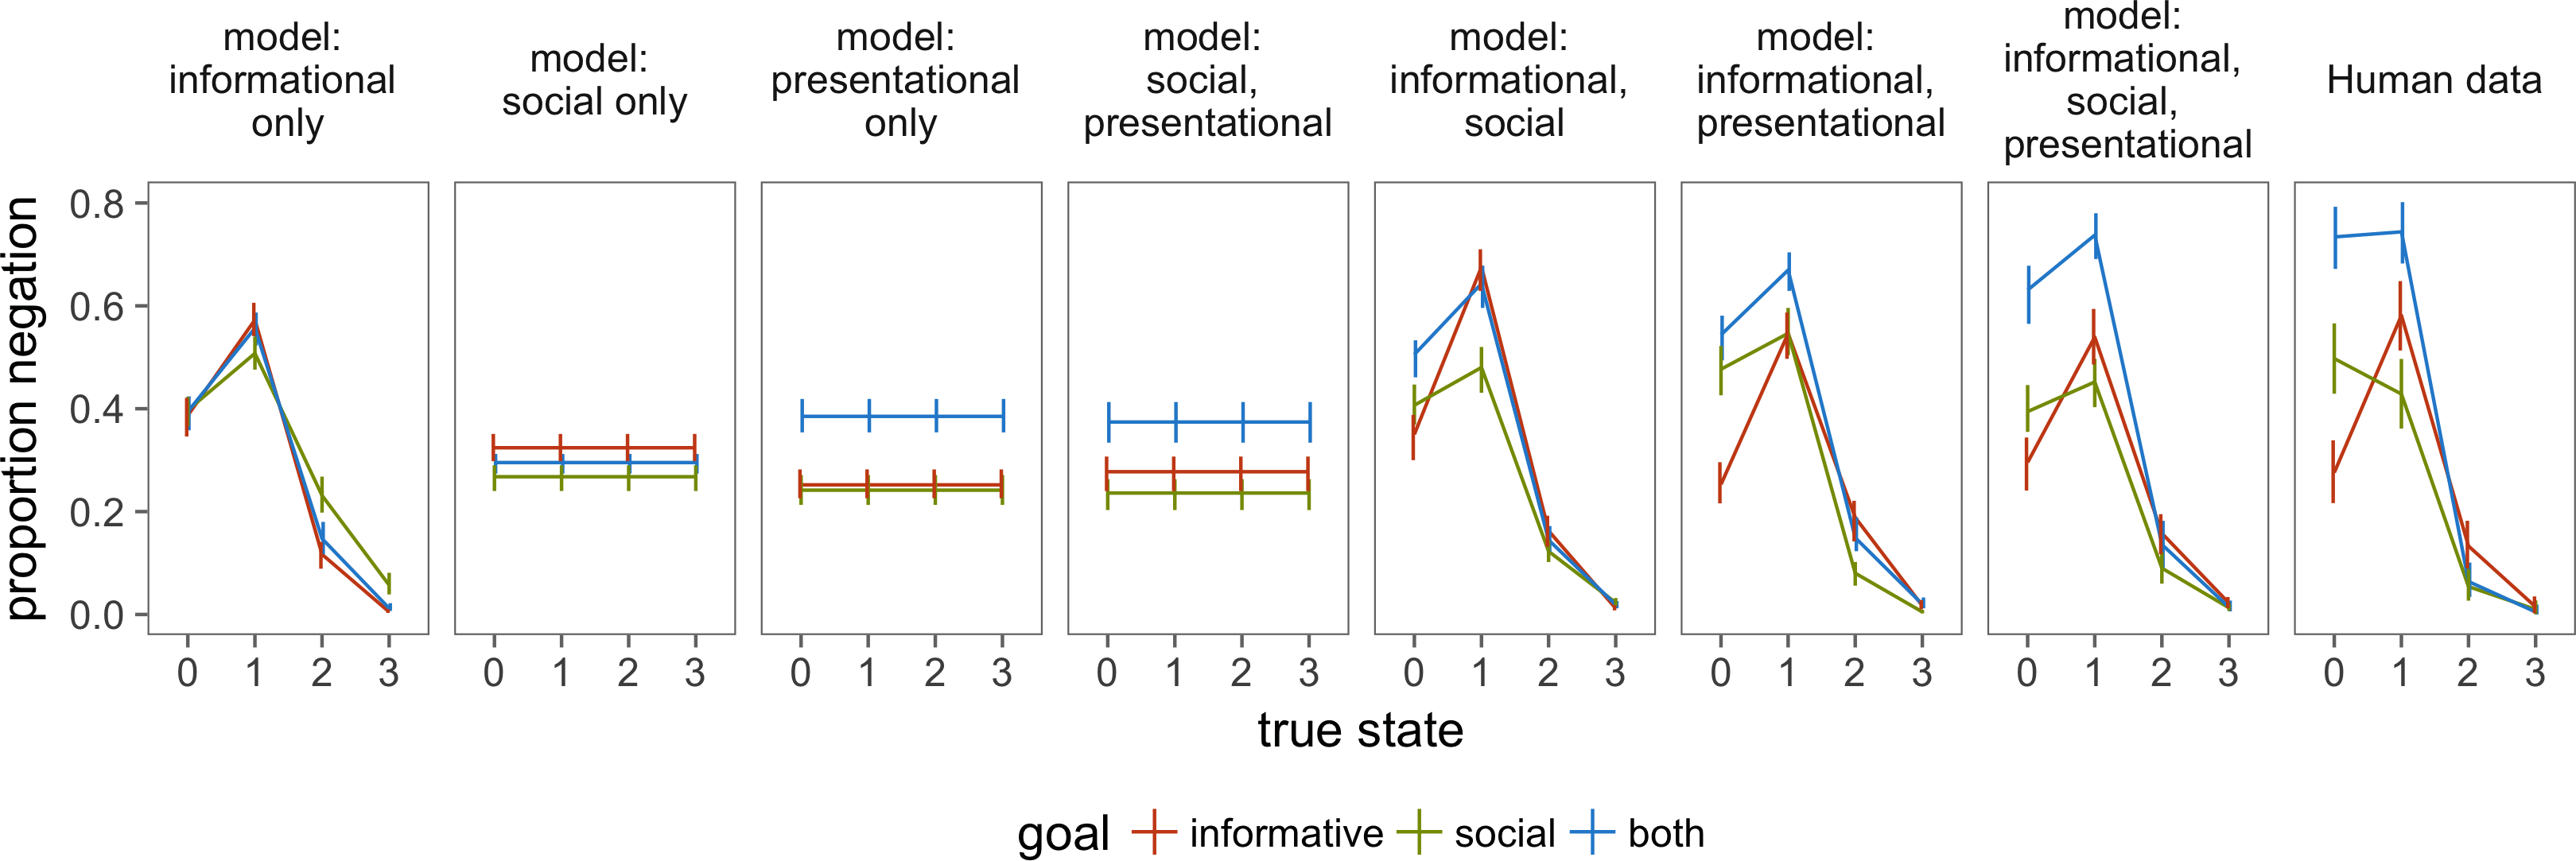
\includegraphics[width=\textwidth]{polite_NHB_files/figure-latex/negation-1} \caption{Experimental results (left) and fitted model predictions (right) for average proportion of negation produced among all utterances, given true states (x-axis) and goals (colors).}\label{fig:negation}
\end{figure}

\newpage

\section{References}\label{references}

\setlength{\parindent}{-0.5in} \setlength{\leftskip}{0.5in}

\hypertarget{refs}{}
\hypertarget{ref-R-ggthemes}{}
Arnold, J. B. (2017). \emph{Ggthemes: Extra themes, scales and geoms for
'ggplot2'}. Retrieved from
\url{https://CRAN.R-project.org/package=ggthemes}

\hypertarget{ref-R-gridExtra}{}
Auguie, B. (2017). \emph{GridExtra: Miscellaneous functions for ``grid''
graphics}. Retrieved from
\url{https://CRAN.R-project.org/package=gridExtra}

\hypertarget{ref-R-papaja}{}
Aust, F., \& Barth, M. (2017). \emph{papaja: Create APA manuscripts with
R Markdown}. Retrieved from \url{https://github.com/crsh/papaja}

\hypertarget{ref-axia1985}{}
Axia, G., \& Baroni, M. R. (1985). Linguistic politeness at different
age levels. \emph{Child Development}, 918--927.

\hypertarget{ref-R-magrittr}{}
Bache, S. M., \& Wickham, H. (2014). \emph{Magrittr: A forward-pipe
operator for r}. Retrieved from
\url{https://CRAN.R-project.org/package=magrittr}

\hypertarget{ref-baker2017rational}{}
Baker, C. L., Jara-Ettinger, J., Saxe, R., \& Tenenbaum, J. B. (2017).
Rational quantitative attribution of beliefs, desires and percepts in
human mentalizing. \emph{Nature Human Behaviour}, \emph{1}(4), 0064.

\hypertarget{ref-baker2009action}{}
Baker, C. L., Saxe, R., \& Tenenbaum, J. B. (2009). Action understanding
as inverse planning. \emph{Cognition}, \emph{113}(3), 329--349.

\hypertarget{ref-barr2013random}{}
Barr, D. J., Levy, R., Scheepers, C., \& Tily, H. J. (2013). Random
effects structure for confirmatory hypothesis testing: Keep it maximal.
\emph{Journal of Memory and Language}, \emph{68}(3), 255--278.

\hypertarget{ref-R-Matrix}{}
Bates, D., \& Maechler, M. (2017). \emph{Matrix: Sparse and dense matrix
classes and methods}. Retrieved from
\url{https://CRAN.R-project.org/package=Matrix}

\hypertarget{ref-R-lme4}{}
Bates, D., Mächler, M., Bolker, B., \& Walker, S. (2015). Fitting linear
mixed-effects models using lme4. \emph{Journal of Statistical Software},
\emph{67}(1), 1--48.
doi:\href{https://doi.org/10.18637/jss.v067.i01}{10.18637/jss.v067.i01}

\hypertarget{ref-R-rwebppl}{}
Braginsky, M., Tessler, M. H., \& Hawkins, R. (n.d.). \emph{Rwebppl: R
interface to webppl}. Retrieved from
\url{https://github.com/mhtess/rwebppl}

\hypertarget{ref-R-langcog}{}
Braginsky, M., Yurovsky, D., \& Frank, M. C. (n.d.). \emph{Langcog:
Language and cognition lab things}. Retrieved from
\url{http://github.com/langcog/langcog}

\hypertarget{ref-brown1987}{}
Brown, P., \& Levinson, S. C. (1987). \emph{Politeness: Some universals
in language usage} (Vol. 4). Cambridge university press.

\hypertarget{ref-buhler1934}{}
Bühler, K. (1934). \emph{Sprachtheorie}. Oxford, England: Fischer.

\hypertarget{ref-R-brms}{}
Bürkner, P.-C. (2017). brms: An R package for bayesian multilevel models
using Stan. \emph{Journal of Statistical Software}, \emph{80}(1), 1--28.
doi:\href{https://doi.org/10.18637/jss.v080.i01}{10.18637/jss.v080.i01}

\hypertarget{ref-clark1980}{}
Clark, H. H., \& Schunk, D. H. (1980). Polite responses to polite
requests. \emph{Cognition}, \emph{8}(2), 111--143.

\hypertarget{ref-R-binom}{}
Dorai-Raj, S. (2014). \emph{Binom: Binomial confidence intervals for
several parameterizations}. Retrieved from
\url{https://CRAN.R-project.org/package=binom}

\hypertarget{ref-R-Rcpp_b}{}
Eddelbuettel, D., \& Balamuta, J. J. (2017). Extending extitR with
extitC++: A Brief Introduction to extitRcpp. \emph{PeerJ Preprints},
\emph{5}, e3188v1.
doi:\href{https://doi.org/10.7287/peerj.preprints.3188v1}{10.7287/peerj.preprints.3188v1}

\hypertarget{ref-R-Rcpp_a}{}
Eddelbuettel, D., \& François, R. (2011). Rcpp: Seamless R and C++
integration. \emph{Journal of Statistical Software}, \emph{40}(8),
1--18.
doi:\href{https://doi.org/10.18637/jss.v040.i08}{10.18637/jss.v040.i08}

\hypertarget{ref-frank2012}{}
Frank, M. C., \& Goodman, N. D. (2012). Predicting pragmatic reasoning
in language games. \emph{Science}, \emph{336}(6084), 998--998.

\hypertarget{ref-gelman2006data}{}
Gelman, A., \& Hill, J. (2006). \emph{Data analysis using regression and
multilevel/hierarchical models}. Cambridge university press.

\hypertarget{ref-goffman1967}{}
Goffman, E. (1967). \emph{Interaction ritual: Essays on face-to-face
interaction}. Aldine.

\hypertarget{ref-goodman2016}{}
Goodman, N. D., \& Frank, M. C. (2016). Pragmatic language
interpretation as probabilistic inference. \emph{Trends in Cognitive
Sciences}, \emph{20}(11), 818--829.

\hypertarget{ref-goodman2013}{}
Goodman, N. D., \& Stuhlmüller, A. (2013). Knowledge and implicature:
Modeling language understanding as social cognition. \emph{Topics in
Cognitive Science}, \emph{5}(1), 173--184.

\hypertarget{ref-dippl}{}
Goodman, N. D., \& Stuhlmüller, A. (2014). The Design and Implementation
of Probabilistic Programming Languages. \url{http://dippl.org}.

\hypertarget{ref-grice1975}{}
Grice, H. P. (1975). Logic and conversation. In P. Cole \& J. L. Morgan
(Eds.), \emph{Syntax and semantics} (Vol. 3, pp. 41--58). Academic
Press.

\hypertarget{ref-hamlin2013mentalistic}{}
Hamlin, K. J., Ullman, T. D., Tenenbaum, J. B., Goodman, N. D., \&
Baker, C. L. (2013). The mentalistic basis of core social cognition:
Experiments in preverbal infants and a computational model.
\emph{Developmental Science}, \emph{16}(2), 209--226.

\hypertarget{ref-R-purrr}{}
Henry, L., \& Wickham, H. (2017). \emph{Purrr: Functional programming
tools}. Retrieved from \url{https://CRAN.R-project.org/package=purrr}

\hypertarget{ref-R-directlabels}{}
Hocking, T. D. (2017). \emph{Directlabels: Direct labels for multicolor
plots}. Retrieved from
\url{https://CRAN.R-project.org/package=directlabels}

\hypertarget{ref-holtgraves1997}{}
Holtgraves, T. (1997). YES, but... positive politeness in conversation
arguments. \emph{Journal of Language and Social Psychology},
\emph{16}(2), 222--239.

\hypertarget{ref-ide1989}{}
Ide, S. (1989). Formal forms and discernment: Two neglected aspects of
universals of linguistic politeness. \emph{Multilingua-Journal of
Cross-Cultural and Interlanguage Communication}, \emph{8}(2-3),
223--248.

\hypertarget{ref-jakobson1960}{}
Jakobson, R. (1960). Linguistics and poetics. In \emph{Style in
language} (pp. 350--377). MA: MIT Press.

\hypertarget{ref-jara2016naive}{}
Jara-Ettinger, J., Gweon, H., Schulz, L. E., \& Tenenbaum, J. B. (2016).
The naïve utility calculus: Computational principles underlying
commonsense psychology. \emph{Trends in Cognitive Sciences},
\emph{20}(8), 589--604.

\hypertarget{ref-kao2015}{}
Kao, J. T., \& Goodman, N. D. (2015). Let's talk (ironically) about the
weather: Modeling verbal irony. In \emph{Proceedings of the 37th annual
conference of the Cognitive Science Society}.

\hypertarget{ref-kao2014}{}
Kao, J. T., Wu, J. Y., Bergen, L., \& Goodman, N. D. (2014). Nonliteral
understanding of number words. \emph{Proceedings of the National Academy
of Sciences}, \emph{111}(33), 12002--12007.

\hypertarget{ref-lassiter2017adjectival}{}
Lassiter, D., \& Goodman, N. D. (2017). Adjectival vagueness in a
bayesian model of interpretation. \emph{Synthese}, \emph{194}(10),
3801--3836.

\hypertarget{ref-lee2014}{}
Lee, M. D., \& Wagenmakers, E. J. (2014). \emph{Bayesian cognitive
modeling: A practical course}. Cambridge Univ. Press.

\hypertarget{ref-leech1983}{}
Leech, G. (1983). \emph{Principles of pragmatics}. London, New York:
Longman Group Ltd.

\hypertarget{ref-liu2017ten}{}
Liu, S., Ullman, T. D., Tenenbaum, J. B., \& Spelke, E. S. (2017).
Ten-month-old infants infer the value of goals from the costs of
actions. \emph{Science}, \emph{358}(6366), 1038--1041.

\hypertarget{ref-R-BayesFactor}{}
Morey, R. D., \& Rouder, J. N. (2015). \emph{BayesFactor: Computation of
bayes factors for common designs}. Retrieved from
\url{https://CRAN.R-project.org/package=BayesFactor}

\hypertarget{ref-R-bindrcpp}{}
Müller, K. (2017a). \emph{Bindrcpp: An 'rcpp' interface to active
bindings}. Retrieved from
\url{https://CRAN.R-project.org/package=bindrcpp}

\hypertarget{ref-R-here}{}
Müller, K. (2017b). \emph{Here: A simpler way to find your files}.
Retrieved from \url{https://CRAN.R-project.org/package=here}

\hypertarget{ref-R-tibble}{}
Müller, K., \& Wickham, H. (2017). \emph{Tibble: Simple data frames}.
Retrieved from \url{https://CRAN.R-project.org/package=tibble}

\hypertarget{ref-R-RColorBrewer}{}
Neuwirth, E. (2014). \emph{RColorBrewer: ColorBrewer palettes}.
Retrieved from \url{https://CRAN.R-project.org/package=RColorBrewer}

\hypertarget{ref-R-jsonlite}{}
Ooms, J. (2014). The jsonlite package: A practical and consistent
mapping between json data and r objects. \emph{arXiv:1403.2805
{[}Stat.CO{]}}. Retrieved from \url{https://arxiv.org/abs/1403.2805}

\hypertarget{ref-pinker2008}{}
Pinker, S., Nowak, M. A., \& Lee, J. J. (2008). The logic of indirect
speech. \emph{Proceedings of the National Academy of Sciences},
\emph{105}(3), 833--838.

\hypertarget{ref-R-coda}{}
Plummer, M., Best, N., Cowles, K., \& Vines, K. (2006). CODA:
Convergence diagnosis and output analysis for mcmc. \emph{R News},
\emph{6}(1), 7--11. Retrieved from
\url{https://journal.r-project.org/archive/}

\hypertarget{ref-R-base}{}
R Core Team. (2017). \emph{R: A language and environment for statistical
computing}. Vienna, Austria: R Foundation for Statistical Computing.
Retrieved from \url{https://www.R-project.org/}

\hypertarget{ref-searle1975}{}
Searle, J. (1975). Indirect speech acts. In P. Cole \& J. L. Morgan
(Eds.), \emph{Syntax and semantics} (Vol. 3, pp. 59--82). Academic
Press.

\hypertarget{ref-shannon1948}{}
Shannon, C. E. (1948). A mathematical theory of communication.
\emph{Bell Syst. Tech. J.}, \emph{27}, 623--656.

\hypertarget{ref-vanRooy2003}{}
Van Rooy, R. (2003). Being polite is a handicap: Towards a game
theoretical analysis of polite linguistic behavior. In \emph{Proceedings
of the 9th conference on theoretical aspects of rationality and
knowledge} (pp. 45--58). ACM.

\hypertarget{ref-R-ggplot2}{}
Wickham, H. (2009). \emph{Ggplot2: Elegant graphics for data analysis}.
Springer-Verlag New York. Retrieved from \url{http://ggplot2.org}

\hypertarget{ref-R-forcats}{}
Wickham, H. (2017a). \emph{Forcats: Tools for working with categorical
variables (factors)}. Retrieved from
\url{https://CRAN.R-project.org/package=forcats}

\hypertarget{ref-R-stringr}{}
Wickham, H. (2017b). \emph{Stringr: Simple, consistent wrappers for
common string operations}. Retrieved from
\url{https://CRAN.R-project.org/package=stringr}

\hypertarget{ref-R-tidyverse}{}
Wickham, H. (2017c). \emph{Tidyverse: Easily install and load the
'tidyverse'}. Retrieved from
\url{https://CRAN.R-project.org/package=tidyverse}

\hypertarget{ref-R-tidyr}{}
Wickham, H., \& Henry, L. (2017). \emph{Tidyr: Easily tidy data with
'spread()' and 'gather()' functions}. Retrieved from
\url{https://CRAN.R-project.org/package=tidyr}

\hypertarget{ref-R-dplyr}{}
Wickham, H., Francois, R., Henry, L., \& Müller, K. (2017). \emph{Dplyr:
A grammar of data manipulation}. Retrieved from
\url{https://CRAN.R-project.org/package=dplyr}

\hypertarget{ref-R-readr}{}
Wickham, H., Hester, J., \& Francois, R. (2017). \emph{Readr: Read
rectangular text data}. Retrieved from
\url{https://CRAN.R-project.org/package=readr}






\end{document}
